\documentclass[10pt,a4paper]{article}

%====================================================
% Page Geometry
%====================================================
\usepackage[
    left=0.70in,
    right=0.70in,
    top=0.78in,
    bottom=0.72in
]{geometry}

%====================================================
% Packages
%====================================================
\usepackage{amsmath,amssymb,amsfonts}
\usepackage{graphicx}
\usepackage{booktabs}
\usepackage{float}
\usepackage{natbib}
\usepackage{siunitx}
\usepackage{xcolor}
\usepackage{titlesec}
\usepackage{microtype}
\usepackage{setspace}
\usepackage{caption}
\usepackage{multicol}
\usepackage{fancyhdr}

%====================================================
% Colours
%====================================================
\definecolor{sectionblue}{RGB}{31,78,121}
\definecolor{subsectionblue}{RGB}{46,95,138}
\definecolor{ruleblue}{RGB}{91,155,213}
\definecolor{citationblue}{RGB}{0,102,178}
\definecolor{urlblue}{RGB}{0,114,188}
\definecolor{textgray}{RGB}{80,80,80}

%====================================================
% Hyperlinks
%====================================================
\usepackage[
    colorlinks=true,
    linkcolor=sectionblue,
    citecolor=citationblue,
    urlcolor=urlblue
]{hyperref}

%====================================================
% Cross-References
%====================================================
\usepackage[
    nameinlink,
    capitalise,
    noabbrev
]{cleveref}

\crefname{equation}{equation}{equations}
\Crefname{equation}{Equation}{Equations}

\crefname{figure}{figure}{figures}
\Crefname{figure}{Figure}{Figures}

\crefname{table}{table}{tables}
\Crefname{table}{Table}{Tables}

%====================================================
% Running Header
%====================================================
\pagestyle{fancy}
\fancyhf{}

\setlength{\headheight}{14pt}

\fancyhead[L]{
    \small\color{textgray}
    Interest Rate Models
}

\fancyhead[R]{
    \small\color{textgray}
    Godfrey Tshehla
}

\fancyfoot[C]{
    \small\color{textgray}
    \thepage
}

\renewcommand{\headrulewidth}{0.4pt}

\renewcommand{\headrule}{
    \hbox to\headwidth{
        \color{ruleblue}
        \leaders\hrule height \headrulewidth\hfill
    }
}

\renewcommand{\footrulewidth}{0pt}

%====================================================
% Section Styling
%====================================================
\titleformat{\section}
  {\large\bfseries\color{sectionblue}}
  {\thesection}
  {0.55em}
  {}
  [\color{ruleblue}\titlerule]

\titleformat{\subsection}
  {\normalsize\bfseries\color{subsectionblue}}
  {\thesubsection}
  {0.55em}
  {}

\titleformat{\subsubsection}
  {\normalsize\bfseries\color{subsectionblue}}
  {\thesubsubsection}
  {0.55em}
  {}

\titlespacing*{\section}
  {0pt}
  {1.4em}
  {0.6em}

\titlespacing*{\subsection}
  {0pt}
  {1.0em}
  {0.4em}

\titlespacing*{\subsubsection}
  {0pt}
  {0.8em}
  {0.3em}

%====================================================
% Two-Column Formatting
%====================================================
\setlength{\columnsep}{0.28in}
\setlength{\columnseprule}{0pt}

%====================================================
% General Formatting
%====================================================
\setstretch{1.02}

\setlength{\parindent}{1em}
\setlength{\parskip}{0pt}

\captionsetup{
    font=small,
    labelfont={bf,color=sectionblue}
}

%====================================================
% Custom Commands
%====================================================
\newcommand{\E}{\mathbb{E}}
\newcommand{\Q}{\mathbb{Q}}
\newcommand{\Var}{\operatorname{Var}}
\newcommand{\dd}{\,\mathrm{d}}

%====================================================
% Equation Numbering
%====================================================
\numberwithin{equation}{section}

%====================================================
% Document
%====================================================
\begin{document}

%====================================================
% Journal-Style Title
%====================================================
\begin{center}

{\color{sectionblue}\rule{\textwidth}{1.2pt}}

\vspace{0.45cm}

{\LARGE\bfseries
A Look at the Ho--Lee Short Rate Model
}

\vspace{0.35cm}

{\large
Godfrey Tshehla
}

\vspace{0.15cm}

{\small
17 October 2026
}

\vspace{0.35cm}

{\color{ruleblue}\rule{\textwidth}{0.6pt}}

\end{center}

\vspace{0.25cm}

%====================================================
% Abstract
%====================================================
\begin{abstract}
\noindent
This paper studies the Ho--Lee short-rate model and its application to
term-structure modelling and interest-rate contingent-claim pricing.
The model is calibrated to an initial term structure through a
time-dependent drift, while interest-rate uncertainty is represented by
a constant volatility parameter. Zero-coupon bonds and European options
on zero-coupon bonds are valued analytically and numerically using Monte
Carlo simulation, finite-difference methods, and a calibrated lattice.
The numerical results are used to assess consistency across valuation
methods and to illustrate the implications of the model's Gaussian
dynamics and absence of mean reversion.
\end{abstract}

\vspace{0.15cm}

\noindent
\textbf{Keywords:}
Ho--Lee model, short-rate model, term structure, zero-coupon bond,
Monte Carlo, finite differences, interest-rate derivatives.

\vspace{0.4cm}

%====================================================
% Begin Two Columns
%====================================================
\begin{multicols}{2}

%====================================================
\section{Introduction}
%====================================================

Short-rate models provide a framework for describing the evolution of
interest rates and valuing securities whose cash flows depend on the term
structure. One of the earliest arbitrage-free term-structure models is
the Ho--Lee model introduced by \citet{HoLee1986}.

The Ho--Lee model specifies the instantaneous short rate under the
risk-neutral measure as a Gaussian process with a time-dependent drift
and constant volatility. Unlike equilibrium short-rate models, the drift
is selected so that the model is consistent with the observed initial
term structure.

The model is particularly useful as a benchmark because of its analytical
tractability and relatively simple calibration. Its principal limitation
is the absence of mean reversion, which causes the variance of the short
rate to increase without bound as the time horizon increases. The
Gaussian specification also permits negative interest rates.

The purpose of this paper is to examine the theoretical and numerical
properties of the Ho--Lee model. Particular attention is given to
term-structure calibration, short-rate dynamics, zero-coupon bond pricing,
and the valuation of a European option on a zero-coupon bond. Analytical
results are compared with Monte Carlo simulation, an implicit
finite-difference method, and a calibrated recombining lattice.

%====================================================
\section{Notation}
%====================================================

The principal notation used throughout the paper is summarised in
\Cref{tab:notation}.

\begin{table}[H]
    \centering

    \caption{
        Principal notation used throughout the paper.
    }
    \label{tab:notation}

    \small
    \renewcommand{\arraystretch}{1.15}

    \begin{tabular}{cl}
        \toprule
        \textbf{Symbol}
        &
        \textbf{Meaning}
        \\
        \midrule
        $r_t$
        & Instantaneous short rate \\
        $\theta(t)$
        & Time-dependent drift \\
        $\sigma$
        & Short-rate volatility \\
        $P(t,T)$
        & ZCB price at time $t$ \\
        $T$
        & Bond maturity \\
        $T_1$
        & Option expiry \\
        $T_2$
        & Underlying ZCB maturity \\
        $X$
        & Strike price \\
        $N$
        & Notional \\
        $\Q$
        & Risk-neutral measure \\
        \bottomrule
    \end{tabular}
\end{table}

%====================================================
\section{The Ho--Lee Model}
%====================================================

Under the risk-neutral probability measure $\Q$, the instantaneous
short rate follows

\begin{align}
    \dd r_t
    &=
    \theta(t)\dd t
    +
    \sigma\dd W_t^{\Q}.
    \label{eq:ho_lee_sde}
\end{align}

Here, $\theta(t)$ is a deterministic time-dependent drift, $\sigma$ is
the constant short-rate volatility, and $W_t^{\Q}$ is a standard
Brownian motion under the risk-neutral measure.

Integrating \Cref{eq:ho_lee_sde} from $0$ to $t$ gives

\begin{align*}
    r_t
    &=
    r_0
    +
    \int_0^t\theta(s)\dd s
    +
    \sigma W_t^{\Q}.
\end{align*}

Since the Brownian component is Gaussian,

\begin{align*}
    r_t
    &\sim
    \mathcal{N}
    \left(
        r_0+\int_0^t\theta(s)\dd s,
        \sigma^2t
    \right).
\end{align*}

The expectation is

\begin{align*}
    \E^{\Q}[r_t]
    &=
    r_0+\int_0^t\theta(s)\dd s,
\end{align*}

while the variance is

\begin{align}
    \Var^{\Q}(r_t)
    &=
    \sigma^2t.
    \label{eq:ho_lee_variance}
\end{align}

As shown in \Cref{eq:ho_lee_variance}, short-rate variance increases
linearly with the time horizon. This behaviour follows directly from the
absence of a mean-reversion term.

%====================================================
\section{Term-Structure Calibration}
%====================================================

Let $P(0,T)$ denote the time-zero price of a zero-coupon bond maturing at
$T$. The instantaneous forward rate is

\begin{align*}
    f(0,T)
    &=
    -\frac{\partial}{\partial T}
    \ln P(0,T).
\end{align*}

To ensure consistency with the initial term structure, the Ho--Lee drift
is specified as

\begin{align}
    \theta(t)
    &=
    \frac{\partial f(0,t)}{\partial t}
    +
    \sigma^2t.
    \label{eq:ho_lee_theta}
\end{align}

Consequently, $\theta(t)$ is determined by the shape of the initial
forward curve and the assumed short-rate volatility rather than being
estimated as an independent constant.

For a continuously compounded zero yield $y(0,T)$,

\begin{align*}
    P(0,T)
    &=
    \exp[-y(0,T)T].
\end{align*}

In the numerical implementation, a smooth parametric zero-yield curve is
used to construct the initial discount curve. The instantaneous forward
curve is then obtained numerically, after which $\theta(t)$ is evaluated
using \Cref{eq:ho_lee_theta}.

%====================================================
\section{Zero-Coupon Bond Pricing}
%====================================================

The time-$t$ value of a zero-coupon bond paying one unit at maturity $T$
is

\begin{align*}
    P(t,T)
    &=
    \E^{\Q}
    \left[
        \left.
        \exp
        \left(
            -\int_t^T r_s\dd s
        \right)
        \right|
        \mathcal{F}_t
    \right].
\end{align*}

Under the calibrated Ho--Lee model,

\begin{align*}
    P(t,T)
    &=
    \frac{P(0,T)}{P(0,t)}
    \exp
    \left[
        -(T-t)(r_t-f(0,t))
    \right.
    \\
    &\qquad\left.
        -\frac{1}{2}\sigma^2t(T-t)^2
    \right].
\end{align*}

The bond price therefore admits the exponential-affine representation

\begin{align*}
    P(t,T)
    &=
    A(t,T)e^{-B(t,T)r_t},
    \\
    B(t,T)
    &=
    T-t.
\end{align*}

At time zero,

\begin{align*}
    P^{HL}(0,T)
    &=
    P^{market}(0,T),
\end{align*}

so the initial term structure is reproduced by construction.

%====================================================
\section{European Option on a Zero-Coupon Bond}
%====================================================

Consider a European option expiring at $T_1$ on a zero-coupon bond
maturing at $T_2$, where

\begin{align*}
    0<T_1<T_2.
\end{align*}

For notional $N$ and strike price $X$, the call payoff at expiry is

\begin{align*}
    C(T_1)
    &=
    N\max(P(T_1,T_2)-X,0).
\end{align*}

The corresponding put payoff is

\begin{align*}
    P_{\mathrm{put}}(T_1)
    &=
    N\max(X-P(T_1,T_2),0).
\end{align*}

At time zero, the integrated forward-bond volatility is

\begin{align*}
    \Sigma
    &=
    \sigma(T_2-T_1)\sqrt{T_1}.
\end{align*}

The time-zero call price is

\begin{align*}
    C(0)
    &=
    N
    \left[
        P(0,T_2)\Phi(d_1)
    \right.
    \\
    &\qquad\left.
        -X P(0,T_1)\Phi(d_2)
    \right],
\end{align*}

where

\begin{align*}
    d_1
    &=
    \frac{
        \ln
        \left(
            \dfrac{P(0,T_2)}
                  {X P(0,T_1)}
        \right)
        +
        \frac{1}{2}\Sigma^2
    }{\Sigma},
    \\
    d_2
    &=
    d_1-\Sigma.
\end{align*}

Here, $\Phi(\cdot)$ denotes the standard normal cumulative distribution
function.

The corresponding put price is

\begin{align*}
    P_{\mathrm{put}}(0)
    &=
    N
    \left[
        X P(0,T_1)\Phi(-d_2)
    \right.
    \\
    &\qquad\left.
        -P(0,T_2)\Phi(-d_1)
    \right].
\end{align*}

Put-call parity gives

\begin{align*}
    C(0)-P_{\mathrm{put}}(0)
    &=
    N
    \left[
        P(0,T_2)
        -
        X P(0,T_1)
    \right].
\end{align*}

The at-the-money forward strike is

\begin{align}
    X_{\mathrm{ATM}}
    &=
    \frac{P(0,T_2)}
         {P(0,T_1)}.
    \label{eq:atm_forward_strike}
\end{align}

%====================================================
\section{Numerical Results}
%====================================================

The numerical experiment uses a short-rate volatility of

\begin{align*}
    \sigma = 0.01,
\end{align*}

and an initial short rate of

\begin{align*}
    r_0 = 0.03.
\end{align*}

The analytical and closed-form solutions provide benchmarks for the
Monte Carlo, implicit finite-difference, and calibrated lattice methods.

%----------------------------------------------------
\subsection{Ho--Lee Lattice}
%----------------------------------------------------

\Cref{fig:ho_lee_lattice} illustrates the recombining short-rate lattice
generated under the Ho--Lee model. The lattice uses
$\sigma=0.01$ and is calibrated to the initial discount curve through
time-dependent level shifts.

\begin{figure}[H]
    \centering
    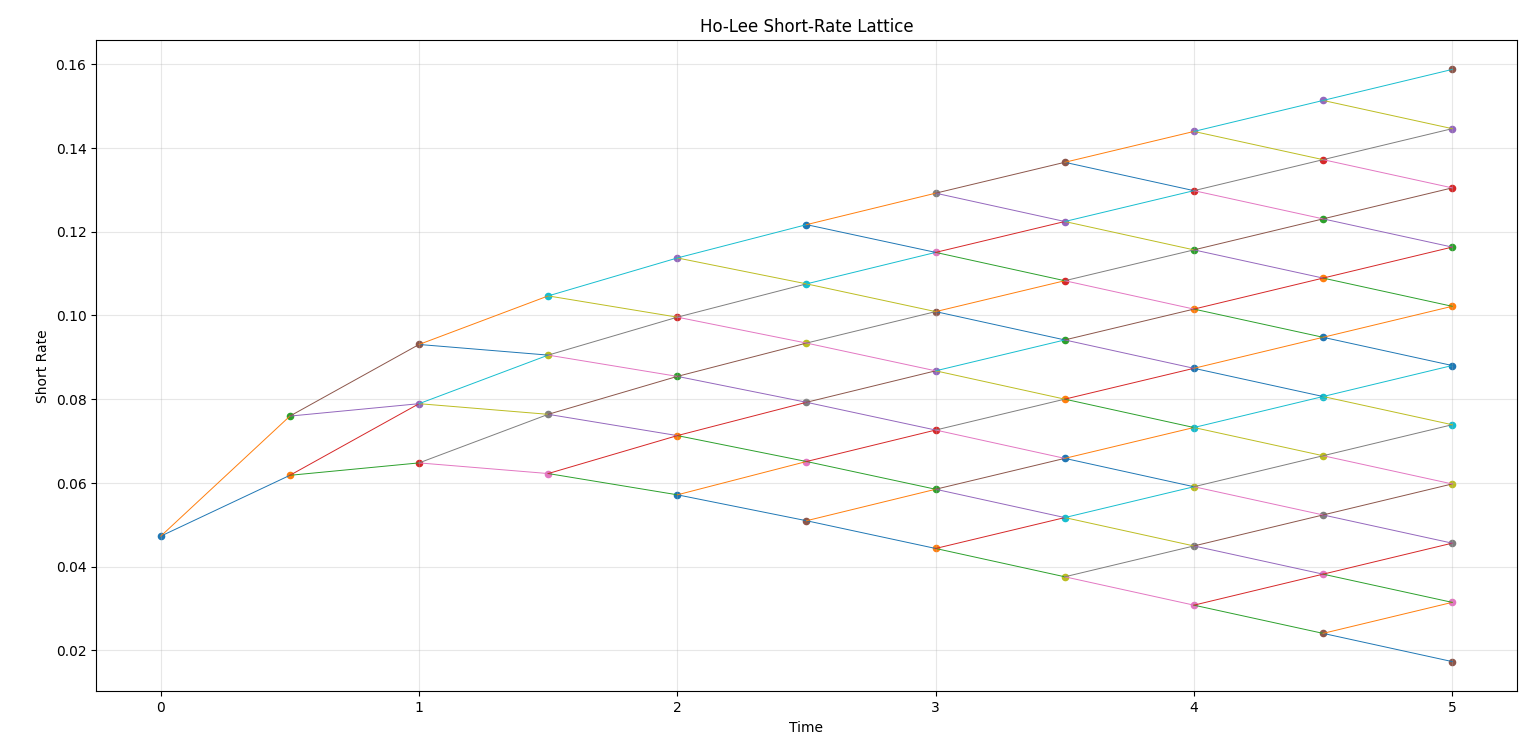
\includegraphics[
        width=0.98\columnwidth
    ]{ho_lee_lattice.png}
    \caption{
        Calibrated recombining Ho--Lee short-rate lattice.
    }
    \label{fig:ho_lee_lattice}
\end{figure}

The lattice displays the characteristic additive structure of the
Ho--Lee model. At each time step, the spacing between adjacent states is
determined by the constant volatility, while the calibrated shift aligns
the tree with the initial term structure.

%----------------------------------------------------
\subsection{Zero-Coupon Bond Results}
%----------------------------------------------------

A five-year zero-coupon bond with unit notional is considered. The market
value implied by the initial discount curve is

\begin{align*}
    P(0,5)
    &=
    0.67188513.
\end{align*}

\Cref{tab:zcb_results} compares the market value with the analytical,
Monte Carlo, implicit finite-difference, and lattice estimates.

\begin{table}[H]
    \centering

    \caption{
        Ho--Lee zero-coupon bond pricing results.
    }
    \label{tab:zcb_results}

    \small
    \renewcommand{\arraystretch}{1.15}

    \begin{tabular}{lcc}
        \toprule
        \textbf{Method}
        &
        \textbf{Price}
        &
        \textbf{Error}
        \\
        \midrule
        Market
        & 0.67188513
        & -- \\
        Analytical
        & 0.67188513
        & $0.000\times10^{0}$ \\
        Monte Carlo
        & 0.67083218
        & $-1.053\times10^{-3}$ \\
        FDM
        & 0.66959218
        & $-2.293\times10^{-3}$ \\
        Lattice
        & 0.67188513
        & $-1.110\times10^{-16}$ \\
        \bottomrule
    \end{tabular}
\end{table}

The analytical price reproduces the market discount factor exactly, as
required by the calibration of the Ho--Lee model. The lattice value also
matches the market price to machine precision because the lattice is
calibrated directly to the initial discount curve.

The Monte Carlo estimate is below the market value by approximately

\begin{align*}
    1.053\times10^{-3},
\end{align*}

whereas the implicit finite-difference estimate differs from the market
value by

\begin{align*}
    -2.293\times10^{-3}.
\end{align*}

The deviations in the Monte Carlo and finite-difference estimates arise
from their numerical approximations rather than from the analytical
term-structure calibration.

%----------------------------------------------------
\subsection{European ZCB Option Results}
%----------------------------------------------------

A European call option expiring at

\begin{align*}
    T_1 = 2
\end{align*}

years is written on a zero-coupon bond maturing at

\begin{align*}
    T_2 = 5
\end{align*}

years. The option has unit notional and uses the at-the-money forward
strike defined in \Cref{eq:atm_forward_strike}. For the initial discount
curve,

\begin{align*}
    X
    &=
    0.77216974.
\end{align*}

The closed-form Ho--Lee price provides the benchmark for the numerical
valuation methods. The results are reported in
\Cref{tab:zcb_option_results}.

\begin{table}[H]
    \centering

    \caption{
        Ho--Lee European zero-coupon bond call option pricing results.
    }
    \label{tab:zcb_option_results}

    \small
    \renewcommand{\arraystretch}{1.15}

    \begin{tabular}{lcc}
        \toprule
        \textbf{Method}
        &
        \textbf{Price}
        &
        \textbf{Error}
        \\
        \midrule
        Closed Form
        & 0.01137126
        & -- \\
        Monte Carlo
        & 0.01124583
        & $-1.254\times10^{-4}$ \\
        FDM
        & 0.01176308
        & $3.918\times10^{-4}$ \\
        Lattice
        & 0.01137831
        & $7.040\times10^{-6}$ \\
        \bottomrule
    \end{tabular}
\end{table}

The lattice estimate is particularly close to the closed-form benchmark,
with an absolute pricing difference of approximately

\begin{align*}
    7.040\times10^{-6}.
\end{align*}

The Monte Carlo estimate differs from the closed-form price by

\begin{align*}
    -1.254\times10^{-4},
\end{align*}

while the implicit finite-difference estimate differs by

\begin{align*}
    3.918\times10^{-4}.
\end{align*}

For the numerical settings used in this experiment, the lattice provides
the closest approximation to the closed-form option value. The
results show consistency between the analytical and numerical valuation
approaches.

%====================================================
\section{Limitations of the Ho--Lee Model}
%====================================================

Despite its tractability, the Ho--Lee model has several important
limitations.

First, the model contains no mean-reversion mechanism. As established in
\Cref{eq:ho_lee_variance},

\begin{align*}
    \Var^{\Q}(r_t)
    &=
    \sigma^2t.
\end{align*}

Consequently,

\begin{align*}
    \lim_{t\rightarrow\infty}
    \Var^{\Q}(r_t)
    &=
    \infty.
\end{align*}

Short-rate uncertainty therefore increases indefinitely with the time
horizon. This behaviour differs from mean-reverting Gaussian models in
which the distribution of the short rate can approach a stationary
long-run variance.

Second, the Gaussian specification assigns positive probability to
negative short rates:

\begin{align*}
    \Pr(r_t<0)
    &>
    0.
\end{align*}

Whether this is economically problematic depends on the application and
interest-rate regime, but it remains an important structural property of
the model.

Third, the model assumes a constant instantaneous volatility $\sigma$.
Although this assumption contributes to analytical tractability, it
restricts the model's ability to reproduce more complex volatility
structures observed in interest-rate markets.

These limitations motivate extensions of the Gaussian short-rate
framework that introduce mean reversion while retaining consistency with
the observed initial term structure \citep{BrigoMercurio2006}.

%====================================================
\section{Conclusion}
%====================================================

The Ho--Lee model provides a simple and tractable arbitrage-free
framework for modelling the term structure of interest rates. Its
deterministic time-dependent drift allows the model to reproduce an
observed initial discount curve, while its Gaussian dynamics lead to
analytically tractable short-rate distributions and zero-coupon bond
prices.

The paper considered the calibration of the model to an initial term
structure and the valuation of a zero-coupon bond and a European option
on a zero-coupon bond. Analytical results were compared with Monte Carlo
simulation, an implicit finite-difference method, and a calibrated
recombining lattice.

For the five-year zero-coupon bond, the analytical and lattice values
reproduced the market discount factor, while the Monte Carlo and
finite-difference methods produced small numerical deviations. For the
European zero-coupon bond call, all three numerical methods produced
values close to the closed-form benchmark, with the lattice giving the
smallest pricing difference for the numerical settings considered.

The simplicity of the Ho--Lee specification is also the source of its
principal limitations. In particular, the absence of mean reversion
causes short-rate variance to increase linearly with time, while the
Gaussian distribution permits negative rates. Nevertheless, the
Ho--Lee model remains an important benchmark for understanding
arbitrage-free term-structure modelling and provides a natural reference
point for more sophisticated short-rate models.

%====================================================
% End Two Columns
%====================================================
\end{multicols}

%====================================================
% References
%====================================================
\bibliographystyle{plainnat}
\bibliography{references}

\end{document}